\documentclass[11pt, a4paper]{exam}
\usepackage{graphicx}
\usepackage[left=0.8in, top=0.7in, total={6.2in,8in}]{geometry}
\usepackage[normalem]{ulem}
\renewcommand\ULthickness{1.0pt}   %%---> For changing thickness of underline
\setlength\ULdepth{1.3ex}%\maxdimen ---> For changing depth of underline
\usepackage[cmex10]{amsmath}

\begin{document}
	%\thispagestyle{empty}
	\noindent
	\begin{minipage}[l]{0.1\textwidth}
		\noindent
		
\includegraphics[width=1.6\textwidth]{figs/logo.png}
	\end{minipage}
\hfill
\begin{minipage}[c]{0.8\textwidth}
	\begin{center}
		\large	Indian Institute of Technology Hyderabad \par
		%\large	Department of Electrical Engineering	\par
		\large	Future Wireless Communitcation \par
	\large \textbf{Entrace Exam}%	\par
%\small	Date: Feb 25, 2020}
	\end{center}
\end{minipage}
\par
\vspace{0.2in}
\noindent
\uline{Duration: 30 min \hfill Date: Jun 23, 2023}%	\hfill Max mark: 10}
\par 
\vspace{0.15in}
\noindent
\centering
%{\small \bfseries 	Attempt any five questions }

\begin{questions}
	\pointsdroppedatright
	\question
	$\overline{AB}$ is parallel to $\overline{ED}$, and the diameter $\overline{EB}$ is parallel to $\overline{DC}$. And $ \cfrac{\angle{AEB}}{\angle{ABE }} = \cfrac{4}{5}$ , then find $\angle{BCD}$.
	\begin{figure}[h!]
	\centering
	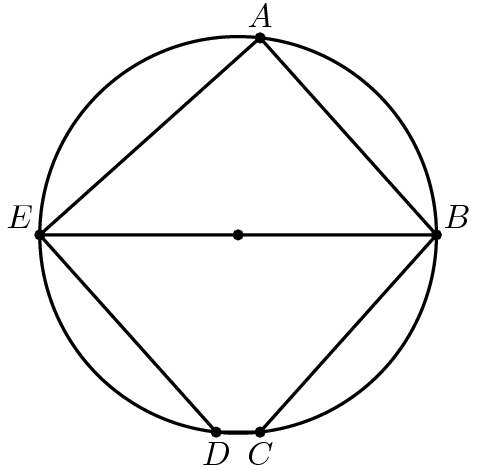
\includegraphics[width=0.27\textwidth]{figs/Q2.png}
	\end{figure}
	%answer = 130

%	\question
%	Prove that the tangent at any point of a circle is perpendicular to the radius through the point of contact.
%	%answer
%	%https://www.toppr.com/ask/question/prove-that-the-tangent-at-any-point-of-a-circle/

%	\question
%	Let $\{a_n\}$ be a non-constant arithmetic progression. $a_1 = 1$ and the following holds true: for any $n \geq 1$, the value of $ \cfrac{a_{2n}+a_{2n-1}+\cdots+a_{n+1}}{a_n+a_{n-1}+\cdots+a_1} $ remains constant (does not depend on $n$). Find $a_{15}$
%	%answer
%	%https://www.math10.com/problems/arithmetic-progression-problems/difficult/

	\question
	If the ratio of the sum of the first $n$ terms of two APs is $\cfrac{5n+31}{7n+17}$ , then find the ratio of their $13^{th}$ terms. 
	%answer = 13/16

\end{questions}
\vspace{0.1in}
{\large \bfseries Best Wishes}
\end{document}
